% Chapter Template

\chapter{Literature Review} % Main chapter title

\label{chp:related} % Change X to a consecutive number; for referencing this chapter elsewhere, use \ref{ChapterX}

Convolutional Neural Network (CNN) outperformed traditional computer vision approaches for medical image classification due to its current advances on architecture design. Typically, CNN architectures are composed of two parts~\cite{krizhevsky2012imagenet}. First part is called a convolutional part which further consists of  convolutional layers interconnected with some connection patterns that are responsible for feature extraction. Second part is the fully connected layers which consist of Dense layers that are responsible for classification. This section discusses previous CNN based CXR classification systems  reporting the modeling mechanisms and the reported results.
\section{CNN Based Models}
In this section CNN base models for covid detection is reviewed.
\subsection{Reliable COVID-19 Detection Using Chest X-ray Images}
\begin{figure}
    \begin{center}
        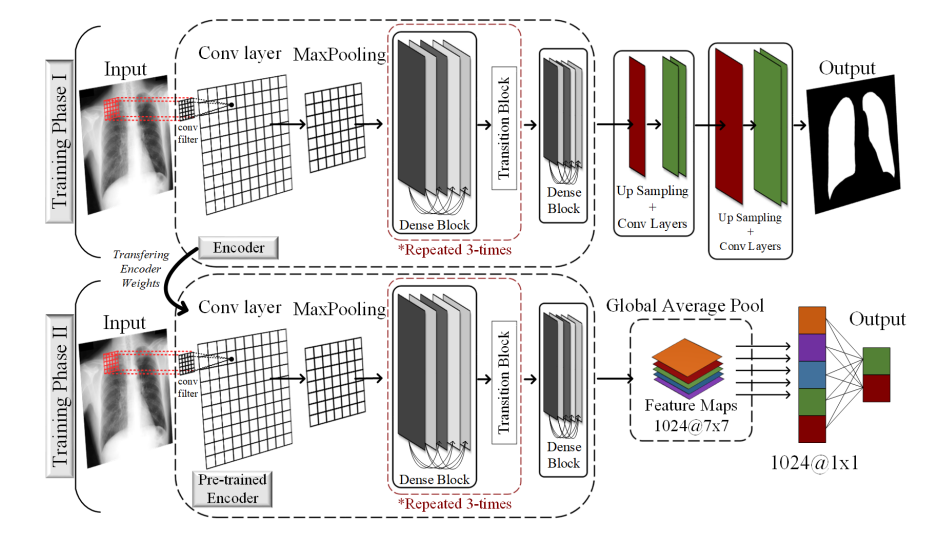
\includegraphics[width=\textwidth]{Figures/RltDag.png}
        \caption{\label{rlt:dag} ReCovNet model proposed by~\cite{dag}. It uses pretrained encoder for classification of COVID-19 CXR image}
    \end{center}
\end{figure}
In \cite{dag}, authors have adapted transfer learning techniques to train CNN models. Training is performed through two phases. Fig.~\ref{rlt:dag} represent proposed system by \cite{dag}. In phase I, u-shaped architecture is excluded by removing the skip connections, which performs the concatenation operation. The reason for constructing an encoder-decoder network without skip connections is that the contributions from the initial layers are avoided; therefore, the network can make decisions from the high level features that are closer to segmentation mapping of the input image.  In phase II, Decoder network is discarded, and the encoder network is fine-tuned for the binary classification task. Adam optimizer is used to train their network. Model is trained with QaTa-COV19 dataset. The method achieved a performance of 98.57\% for sensitivity and 99.77\%  for specificity.

\subsection{Advance Warning Methodologies for
COVID-19 Using Chest X-Ray Images}

% In \cite{ar}, authors have proposed Convolutional Support Estimator Networks (CSENs) classifier. CSEN is used to classify features extracted by DenseNet-121. DenseNet-121 is pre-trained using ImageNet Dataset then fine-tuned using QaTa-Cov19. CSEN achieved 97\% of sensitivity and over 95.5\% of specificity. Authors also evaluated DenseNet-121 achieving 95\% of  sensitivity and 99.74\% of specificity.

In \cite{ar}, authors evaluated the performance of different classifier for classifying the feature produced by DenseNet121. Their methedology is as follows:
\subsubsection{Feature Extraction using DensNet121}
They pretrained two DenseNet121~\cite{huang2017densely} models on Early-QaTa-COV19 and ChestX-ray14 datasets are used to extract 1024-D feature vectors by taking the output after global pooling just before the classification layer. Then, a dimensionality reduction is applied over the calculated features with principal component analysis (PCA) by choosing the first $512$ principal components.

\subsubsection{Representation-based classification}
 Representation-based classification (RC) techniques are used in many different classification tasks such as face recognition in~\cite{wright2010sparse}, hyperspectral image classification~\cite{li2016survey}, and human action recognition~\cite{guha2011learning}. Authors classified the feature vector produced by DenseNet121 using either Sparse RC or Collaborative RC. It is performed as follows:
 \begin{equation}
    \begin{split}
        \hat{x} = \arg \min_{x}(\lambda \vert \vert x \vert\vert_{1} + \vert\vert y - Dx \vert\vert_{2})
    \end{split}
\end{equation}
where $D$ is the dictionary of feature produced by DenseNet121 and projected using PCA. Sparse RC minimizes $\ell^{1}$ of $\hat{x}$. While Collaborative RC minimizes $\ell^{2}$ of $\hat{x}$ as follows:
\begin{equation}
    \begin{split}
        \hat{x} = \arg \min_{x}(\lambda \vert \vert x \vert\vert_{2} + \vert\vert y - Dx \vert\vert_{2})
    \end{split}
\end{equation}
For both types of representations $\hat{x}$ reconstruction error is calculated as follows:
\begin{equation}
    \begin{split}
        e_i = \vert\vert y - D\hat{x} \vert\vert_2
    \end{split}
\end{equation}
Then assign a class of the lower construction error as follows:
\begin{equation}
    \begin{split}
        class(y) \arg \min(e_i)
    \end{split}
\end{equation}

Fig.~\ref{fig:RC} represent representation classification pipeline presented in~\cite{ar}. They achieved a $.98$ and $.97$ of accuracy for Sparse Representation-based classification and Collaborative Representation-based classification, respectively. 
\begin{figure}
    \centering
    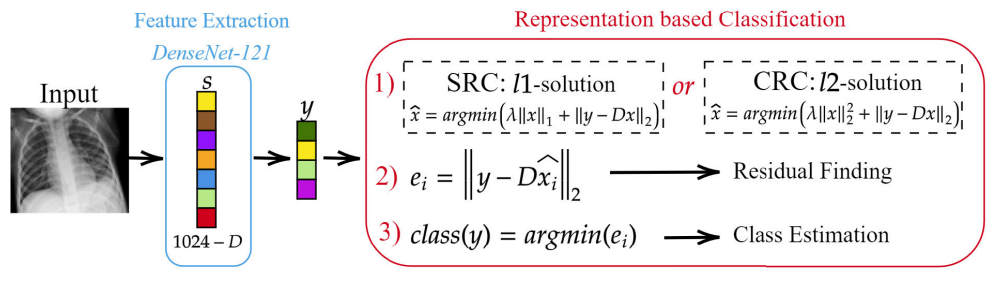
\includegraphics[width=\textwidth]{Figures/RCpipline.png}
    \caption{\label{fig:RC} sparse and Collaborative Representation learning pipeline of~\cite{ar}}
\end{figure}
Authors of~\cite{ar} also evaluated SVM for classifying features produces by DenseNet121 and recorded $.98$ of accuarcy.

%  \begin{algorithm}[H]
%     \DontPrintSemicolon
%     \caption{Sparse Representation-based Classification (SRC)}
%     \KwIn{a matrix of training samples $A = [A_{1}, A_{2}, \dots ,A_{k}] \in \mathbb{R}^{m \times n}$ 
%       for $k$ classes, a test sample $\mathbf{y} \in \mathbb{R}^{m}$, (and an optional error tolerance $\varepsilon > 0$).}
%     Normalize the columns of $A$ to have unit $\ell^{2}$-norm.\;
%     Solve the $\ell^{1}$-minimization problem:
%     $\hat{\bm{x}}_{1} = \arg \min_{x}\norm{\bm{x}}_{1}\quad \text{subject to}\quad A\bm{x} = \bm{y}$ \;
%     (Or alternatively, solve
%     $\hat{\bm{x}}_{1} = \arg \min_{x}\norm{\bm{x}}_{1}\quad \text{subject to}\quad \norm{A\bm{x} = \bm{y}}_{2} \leqslant \varepsilon$).\;
%     Compute the residuals $r_{i}(\bm{y}) = \norm{\bm{y} - A \delta_{i}(\hat{\bm{x}}_{1})}_{2}$\;
%     \For{$i = 1,\dots,k$}{something}
%   \end{algorithm}
  
\subsection{COVID-19 Detection Using DL Algorithm on CXR Images}

In~\cite{akt}, authors proposed a modified MobileNetV2 CNN model where the stander convolution is replaced by a depth-wise convolution. Their model is trained with $3616$ COVID-19 CXR images and 10,192 normal CXR images. Dataset is initially preprocessed by reshaping input images to $299\times299$ and image enhancement technique is applied. The model achieved an accuracy of 98\% for binary classification task. Fig.~\ref{fig:akterPipeline} illustrates general pipeline proposed by~\cite{akt} which is detailed as follows:

\begin{figure}
    \begin{center}
        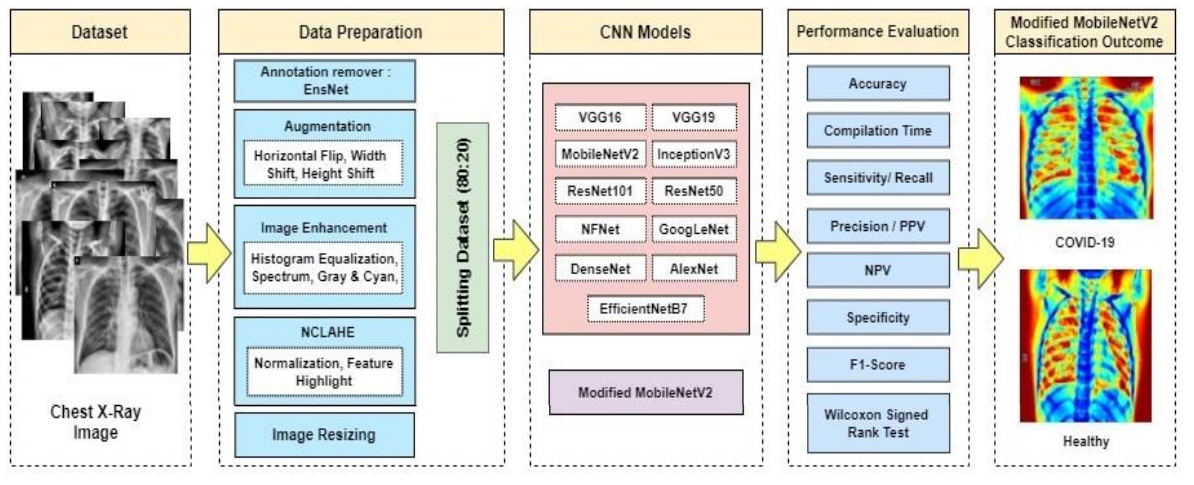
\includegraphics[width=\textwidth]{Figures/AkterPipeline.png}
        \caption{\label{fig:akterPipeline} Pipeline proposed in~\cite{akt} for COVID-19 classification}
    \end{center}
\end{figure}

Preprocessing phase of~\cite{akt} initially performs image augmentations which includes horizontal flip, rotation, width shift and height shift on all the extracted data from the original dataset. Also, image enhancement applied Histogram equalization, Spectrum, Grays and Cyan. The N-CLAHE algorithm was then used to normalize pictures and highlight smaller features for machine learning classifiers to notice. Thereafter, the images were resized to the classifier’s standard resolution. After resizing the picture, the machine learning classifier used the enhanced (52,000) images in a ratio of 80\% data for training, whereas 20\% was used for testing. They proposed modified MobileNetV2 network and achieved 98\% of accuracy

\section{Traditional Computer Vision Models}
\subsection{ COVID-19 detection in CXR images using
majority voting based classifier ensemble}

In~\cite{acos}, authors proposed a two phases COVID-19 multi-label classification system as illustrated in Fig.~\ref{fig:Acos}. The system phase I classifies the input CXR images as normal or COVID-19. In case the image  is classified as COVID-19, phase II further classifies this image as pneumonia or COVID-19. Phase I and Phase II have the same structure with a total of $8196$  local features are extracted then classified using ensemble module. Base classifier of the ensemble module consist of NB, ANN, DT and SVM. A majority voting is used to combine the predictions of these classifiers. Their system achieved accuracy of $98.062$\%  and $91.329$\% for Phase I and Phase II, respectively. Both Phases have same anatomy of preprocessing and feature Description.
\begin{figure}
    \begin{center}
        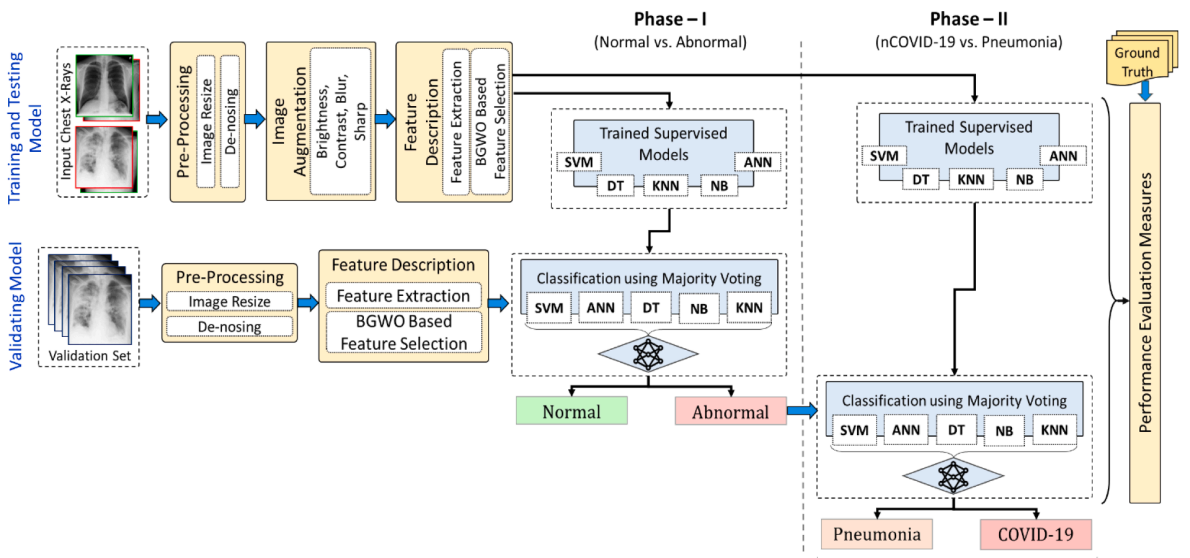
\includegraphics[width=\textwidth]{Figures/ACoS.png}
        \caption{\label{fig:Acos} Proposed machine learning pipeline of~\cite{acos}}
    \end{center}
\end{figure}
Feature extraction is performed by extracting a total of 8196 features as follows:
\begin{itemize}
    \item 8 features using FOSF~\cite{srinivasan2008statistical}.
    \item 88 feature using GLCM~\cite{gomez2012analysis}.
    \item 8100 feature using HOG~\cite{dalal2005histograms}.
\end{itemize}
binary grey wolf optimization (BGWO)~\cite{mirjalili2014grey} is to select the most relavant features from the previously extacted features. The final prediction of the set is the majority vote of seven benchmark classifiers (ANN, KNN, NB, DT, SVM (linear kernel, radial basis function (RBF) kernel, and polynomial kernel).


In \cite{hyp} authors have proposed a hybrid model for multilabel classification where VGG16 is used as a feature extractor. Their system is trained by a combined dataset of QaTaCov19 and Chest X-Ray achieving accuracy of $91.09$\%.

Despite the high accuracy of current CNN based CXR classification methods, but these methods don't address the problem that CNN is scale variant model. This problem hinders the recognition of large scale COVID-19 pneumonia. In this paper, a novel scale-invariant CNN architecture is proposed for classification of COVID-19 pneumonia. The proposed architecture deploys Atrous convolution method for learning the scale-invariant features. Then, an attention model is utilized to automatically and internally select at which scale  CNN should consider and ignore other scales. The proposed architecture exploits texture augmentation to reduce the overfitting and artificially enlarge the training dataset. The experimental results show that proposed system outperforms  the previous  CNN based CXR classification methods  with lower trainable parameter number.


\begin{table}[htbp]
\caption{\label{tbl:related}Overview of recent studies for classifying COVID19}
\begin{center}
\begin{adjustbox}{angle=90}
\begin{tabular}{|l|r|r|l|l|l|}%{lrrlll}
\hline
Work &  \#Samples &  Classes &  Model &  Best Performing Model &   Performance \\
\hline
\hline
~\cite{35apostolopoulos2020covid} & 1428 &    3 & VGG19, MobileNetV2, &   MobileNetV2 & Acc = 96.78\%  \\

      &      &    & Inception, Xception &    &   \\
\hline
~\cite{36hall2020finding} &  204 &    2 &   VGG16 + Resnet50 & VGG16 + Resnet50, &    Acc = 89.2\% \\

     &    &      &                        &   custom CNN &      \\
\hline           
~\cite{37narin2021automatic} &  100 &    2 &   ResNet50, InceptionV3, &  ResNet50 &  Acc = 98\% \\

&    &      &   and InceptionRes-NetV2 &   &    \\
\hline
~\cite{38tang2020automated} &    21152 &    2 &    CNN &   CNN &   Acc = 94.64\% \\
\hline
~\cite{39minaee2020deep}  & 5184 &    2 &   ResNet18, ResNet50, &    SqueezeNet & Sensitivity = 98\%\\

  &   &      &     SqueezeNet, DenseNet-121 &      &  \\
\hline
~\cite{40afshar2020covid}  &    13975 &    2 & COVID-CAPS &    COVID-CAPS &   Acc = 95.7\%, \\
\hline
~\cite{41ahsan2020covid}  &  400 &    2 & VGG16, InceptionResNetV2, &  NasNetMobile &   Acc = 93.94\% \\

  &    &      &  ResNet50, DenseNet201  &    &     \\
\hline
~\cite{42hemdan2020covidx}  &   75 &    2 & VGG19, Xception,  &   VGG19, DenseNet &   F1 scores = 0.91 \\

  &     &      &  ResNetV2, DenseNet201 &     &    \\
\hline
~\cite{43ozturk2020automated}  & 1127 &    2 &   Modified Darknet &  Modified Darknet &  Acc = 98\% \\
\hline
~\cite{44khan2020coronet}  & 1257 &    3 &   Xception &  Xception &  Acc = 94\% \\
\hline
~\cite{45chandra2021coronavirus} & 2356 &    3 &    ACoS system &  ACoS &   Acc = 91.33\% \\
\hline
~\cite{46sekeroglu2020covid19} & 6100 &    3 & SVM, LR, DT, &   Mean result &    Acc = 98.5\% \\

  &   &      &   kNN + VGG16,  &    &    \\

  &   &      &    ResNet50 &    &    \\
\hline
~\cite{47pandit2021automatic}& 1428 &    2 &  VGG16 & VGG16 &  Acc = 96\% \\
\hline
~\cite{48arias2020artificial} &    79500 &    3 &   Grad-CAM &  Grad-CAM &    Acc = 91.5\% \\
\hline
~\cite{49yamac2021convolutional} & 6200 &    4 &  CSEN-based classifier & CSEN-based Classifier &    Sensitivity = 98\% \\
\hline
~\cite{50wang2020covid} &    13975 &   19 &  COVID-Net & COVID-Net &    Acc = 93.3\% \\
\hline
~\cite{51abbas2021classification} &  196 &    3 & DeTrac &    Detrac &    Acc = 93.1\% \\
\hline
~\cite{52toraman2020convolutional} & 3150 &    3 &    CapsNet &   CapsNet &  Acc = 97\% \\
\hline
~\cite{53das2022automated} & 1127 &    3 &   Xception &  Xception &  Acc = 97\% \\
\hline
~\cite{54hu2020learning} & 7470 &    2 &    MD-Conv &   MD-Conv &    Acc = 93.4\% \\
\hline
~\cite{55ismael2021deep} &  380 &    2 &    Novel CNN Model &   Novel CNN Model &    Acc = 91.6\% \\
\hline
~\cite{56shankar2021optimal} &  247 &    2 &   BMO-CRNN &  BMO-CRNN &  Acc = 97.31\% \\
\hline
\end{tabular}
\end{adjustbox}
\end{center}
\end{table}

